\clearpage
\subsection{Library} % (fold)
\label{sub:library}

A library is a collection of reusable code artefacts. Each programming language has its own library, and your programs can make use of the code available in this library.

\begin{figure}[h]
   \centering
   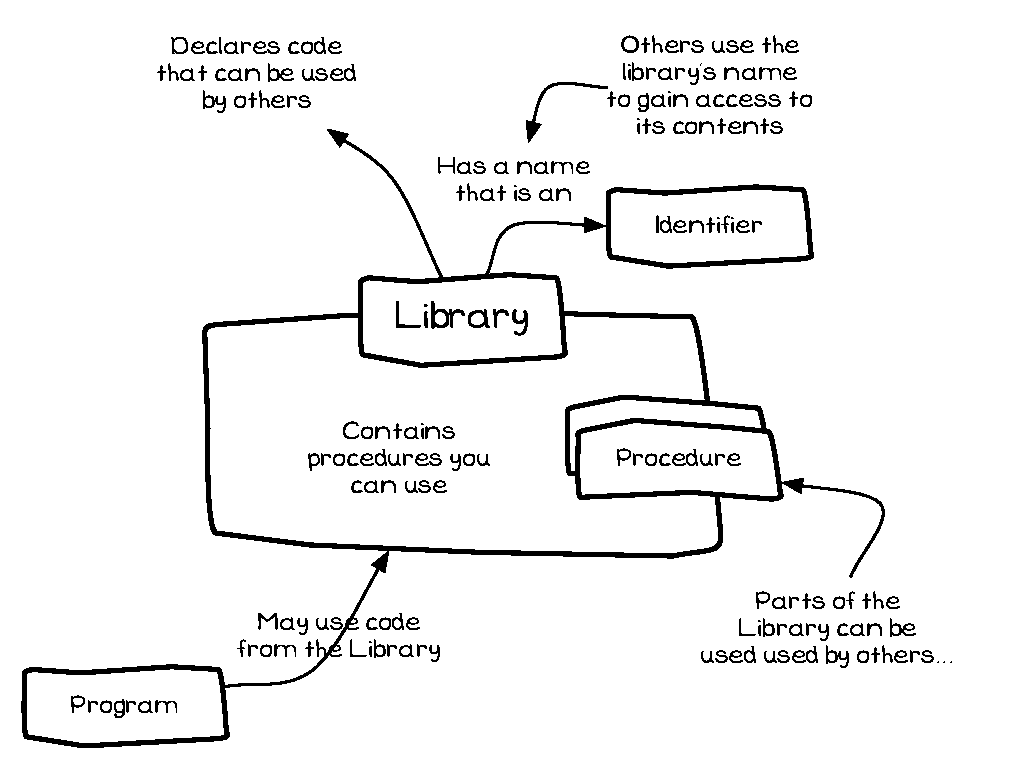
\includegraphics[width=\textwidth]{./topics/program-creation/diagrams/Library} 
   \caption{A library contains code that can be used by your Program}
   \label{fig:program-creation-library}
\end{figure}


\mynote{
\begin{itemize}
  \item A library is an \textbf{artefact}, it contains reusable artefacts.
  \item Figure \ref{fig:program-creation-library} shows the concepts related to a library.
  \item A library is a collection of reusable code artefacts that you can use to perform certain tasks.
  \item The library will contain \nameref{sub:procedure}s that perform a number of tasks.
  \item Each language has a standard library with code to perform many commonly performed tasks.
  \item Other libraries extend the capability of the languages further.
  \item SwinGame is a external library containing code to help you build games.
\end{itemize}
}

% section program (end)